\documentclass{beamer}
\usepackage[latin1]{inputenc}
\usepackage{amsfonts}
\usepackage{epsfig}
\usepackage{hyperref}
\usepackage{multicol}
\usepackage{graphicx}
\usetheme{Warsaw}
\title[The Tempest \hspace{15em} \insertframenumber / \inserttotalframenumber]{Colonization in The Tempest and its Afterlives}

\author {Ravi Bhoraskar}
\begin{document}
\begin{frame}[plain]
\titlepage
\begin{center}
\begin{figure}[htp]
  \begin{center}
    \centering
    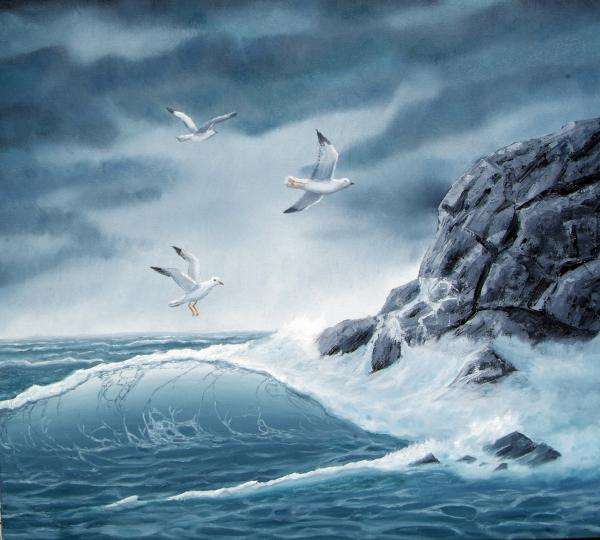
\includegraphics[scale=0.17]{title.jpg}
  \end{center}
\end{figure}
under guidance of\\
Prof. Sudha Shastri\\
IIT Bombay
\end{center}
\end{frame}
\begin{frame}{Outline}
  \begin{multicols}{2}
  \tableofcontents  
  \end{multicols}
\end{frame}
\section{Introduction}
\subsection{A brief history of Colonization}
\begin{frame}{A brief history of British Colonization}
  \begin{columns}[c]
    \column{.6\textwidth}
  \begin{itemize}
  \item \textbf{1492} Columbus discovered America (mistook it for India)
  \item \textbf{1497} Henry VII commissions John Cabot; First Englishman in America
   %No colonization so far, just trade. John Cabot's ship disappeared in his second voyage.
  \item \textbf{1576 onwards} Early claims of land in the name of queen
  \item \textbf{1607} Colonization of America started, with \emph{Virginia Company} creating colony at Jamestown, Virginia
    %Parallels with the colonial discourse prophetic, rather than descriptive
  \end{itemize}
  \column{.4\textwidth}
    \begin{figure}[htp]
      \begin{center}
        \centering
        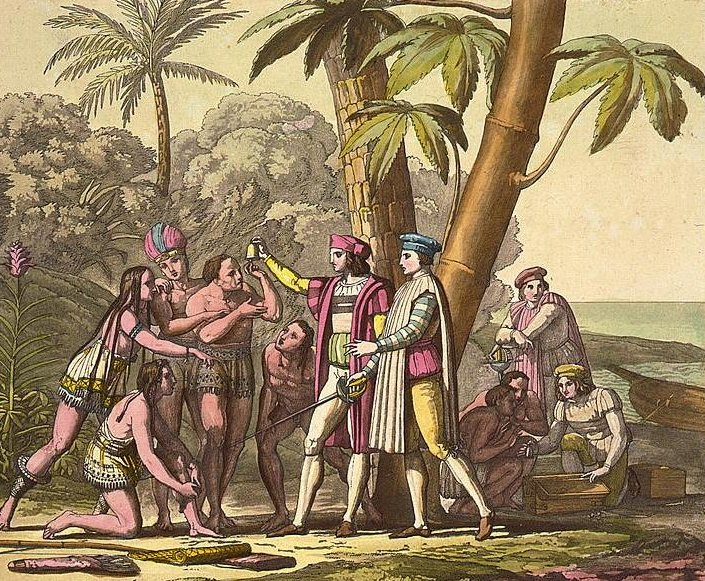
\includegraphics[scale=0.29]{columbus.jpg}
      \end{center}
    \end{figure}
    \end{columns}
\end{frame}

\begin{frame}{The Sea Venture incident}
  \begin{columns}[c]
    \column{.4\textwidth}
    \begin{figure}[htp]
      \begin{center}
        \centering
        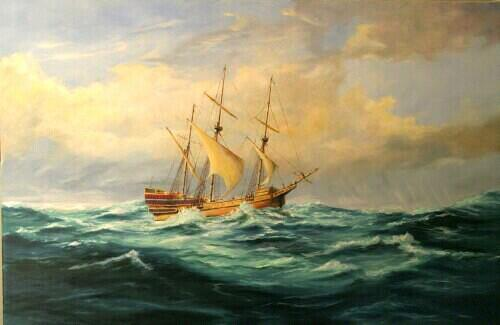
\includegraphics[scale=0.29]{seaventure.jpg}
      \end{center}
    \end{figure}
    \footnotesize{\emph{The Sea Venture in a heavy Sea in 1609,} painting by Christopher Grimes}
    \column{.6\textwidth}

  \begin{itemize}
  \item \emph{Sea Venture} commissioned in 1609 to deliver supplies to the Jamestown colony
  \item Set sail on June 20; Ran into storm and sank on July 24
  \item All 150 passengers land safely ashore, onto a reef in Bermuda
  \item Stranded for 9 months; built 2 new boats; sailed to Virginia; most saved
  \item William Strachey wrote accounts, which supposedly inspired The Tempest
  \end{itemize}
  \end{columns}
\end{frame}

% \subsection{The Tempest}
\begin{frame}{The Tempest}
  \begin{enumerate}
    \item Shakespeare's last play; written in 1610-11
    \item Prospero, Miranda, Ariel, Caliban
    \item Themes
  \end{enumerate}
\end{frame}

\begin{frame}{The Tempest}
  Show video: The Tempest in a minute
\end{frame}


\end{document}
